%% This is the analysis.tex file

Time for some analysis, and probably graphs and tables. Thankfully
\LaTeX{} (and \LaTeXe{}) provides very nice environments for both.

\section{Preliminary Analysis}
\begin{figure}[t]
\begin{center}
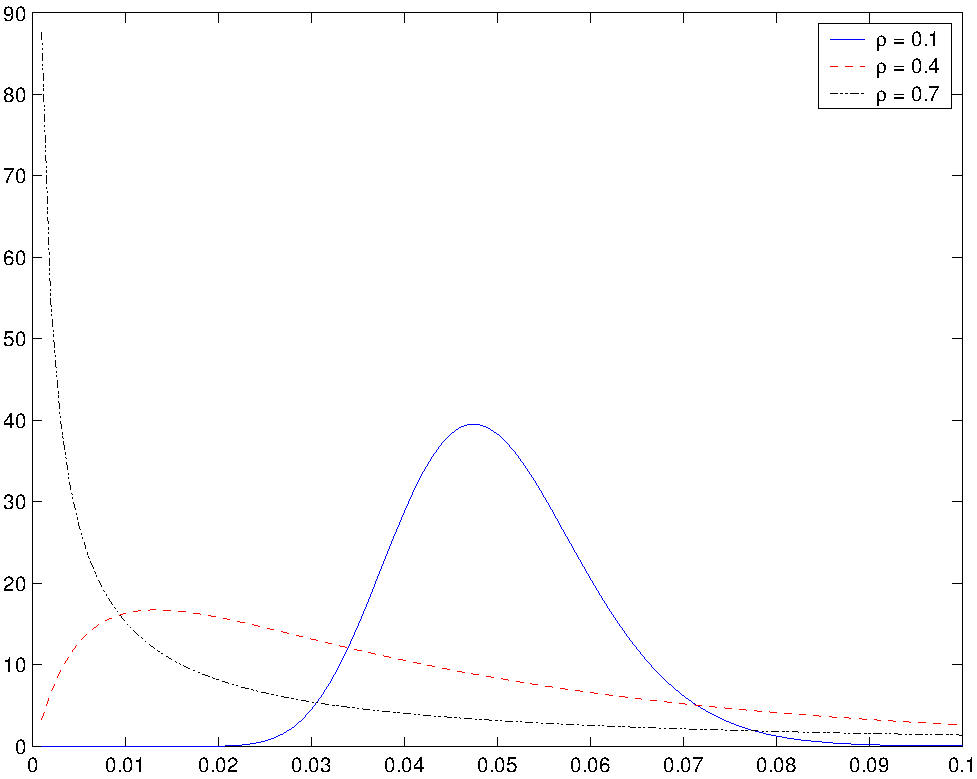
\includegraphics[width=0.8\textwidth]{./Figures/dens.pdf}
\caption{The density function $f$ as given in \eqref{density} for
  three different $\rho$'s and $\bar{p} = 0.05$. (Plotted on $[0,
  0.1]$ for convenience.)}
\label{fig:dens}
\end{center}
\end{figure}
Assume that the random variable $D$ given $\tilde{p} = p$ is
binomially distributed with parameters 50 and $p$ (probability of
success, in this case default). We also take the cumulative
distribution function of $\tilde{p}$ to be
\begin{equation*}
F(\theta) = \P\{\tilde{p} \le \theta\} = \Phi \left( \frac{1}{\rho}
\left(\sqrt{1 - \rho^2}\, \Phi^{-1}(\theta) - \Phi^{-1}(\bar{p})
\right) \right)
\end{equation*}
where $\Phi$ is the cumulative standard normal distribution
function, $\rho$ is the correlation coefficient between the
idiosyncratic and market factors and $\bar{p}$ is the mean default
probability ($\bar{p} = \E \tilde{p}$). To calculate the density of
$\tilde{p}$ let
\begin{eqnarray*}
h(\theta, \rho, \bar{p}) &:=& \frac{1}{\rho} \left(\sqrt{1 -
\rho^2}\, \Phi^{-1}(\theta) - \Phi^{-1}(\bar{p}) \right), \\
\varphi(\theta) &:=& \frac{d}{d \theta} \Phi(\theta) =
\frac{1}{\sqrt{2 \pi}} e^{- \theta^2/2},
\end{eqnarray*}
and notice that since $\Phi$ is a bijection we have
\[\Phi \circ \Phi^{-1}(\theta) = \Phi^{-1} \circ \Phi(\theta) =
\theta, \] for every $\theta \in \R$. Then, we have for the density
of $\tilde{p}$,
\begin{eqnarray}
f(\theta, \rho, \bar{p}) &=& \frac{d}{d \theta} F(\theta) =
\Phi'(h(\theta, \rho, \bar{p})) \frac{\pa}{\pa \theta} h(\theta,
\rho, \bar{p}) \nonumber \\
&=& \varphi(h(\theta, \rho, \bar{p})) \frac{\sqrt{1 -
\rho^2}}{\rho} \frac{d}{d \theta} \Phi^{-1}(\theta) \nonumber \\
&=& \varphi(h(\theta, \rho, \bar{p})) \frac{\sqrt{1 - \rho^2}}{\rho}
\frac{1}{\varphi (\Phi^{-1}(\theta))}, \label{density}
\end{eqnarray}
for $\theta \in (0,1)$ and zero otherwise, since
\begin{eqnarray*}
\frac{d}{d \theta} \left(\Phi (\Phi^{-1}(\theta)) \right) &=&
\Phi'(\Phi^{-1}(\theta)) \frac{d}{d \theta} \Phi^{-1}(\theta)
\Leftrightarrow \\
\frac{d}{d \theta} \theta &=& \varphi(\Phi^{-1}(\theta))
\frac{d}{d \theta} \Phi^{-1}(\theta) \Leftrightarrow \\
\frac{d}{d \theta} \Phi^{-1}(\theta) &=&
\frac{1}{\varphi(\Phi^{-1}(\theta))}.
\end{eqnarray*}



The density of $\tilde{p}$ is shown in Figure \ref{fig:dens} for
three different values of $\rho$ and $\bar{p} = 0.05$. The effect of
the correlation is to put more mass towards higher default
probabilities as the correlation increases, thus resulting in larger
number of defaults as the correlation increases.

\begin{table}[htbp]
\caption{Values of the CDO Tranches.} \label{tab:cdo}
\begin{center}
\begin{tabular}{lllll}
\hline \hline
&            &             \multicolumn{ 3}{c}{$\rho$} \\
\hline
&            &       0.1 &        0.4 &        0.7 \\
\hline Equity &        $C_E^\star(T)$ &     2.5712 &     2.8957 &
3.5642 \\
Junior &        $C_J^\star(T)$ &     9.9289 &     9.6137 &
9.2120 \\
Senior &        $C_S^\star(T)$ &    35.0000 &    34.9905 &
34.7239 \\
\hline Sum & $C_E^\star(T) + C_J^\star(T) + C_S^\star(T)$ & 47.5000&
47.5000 &  47.5001 \\
\hline \hline
\end{tabular}
\end{center}
\end{table}
Using the default values for the parameters as above we get the
values for the tranches in Table~\ref{tab:cdo}.

\begin{figure}[thbp]
\begin{center}
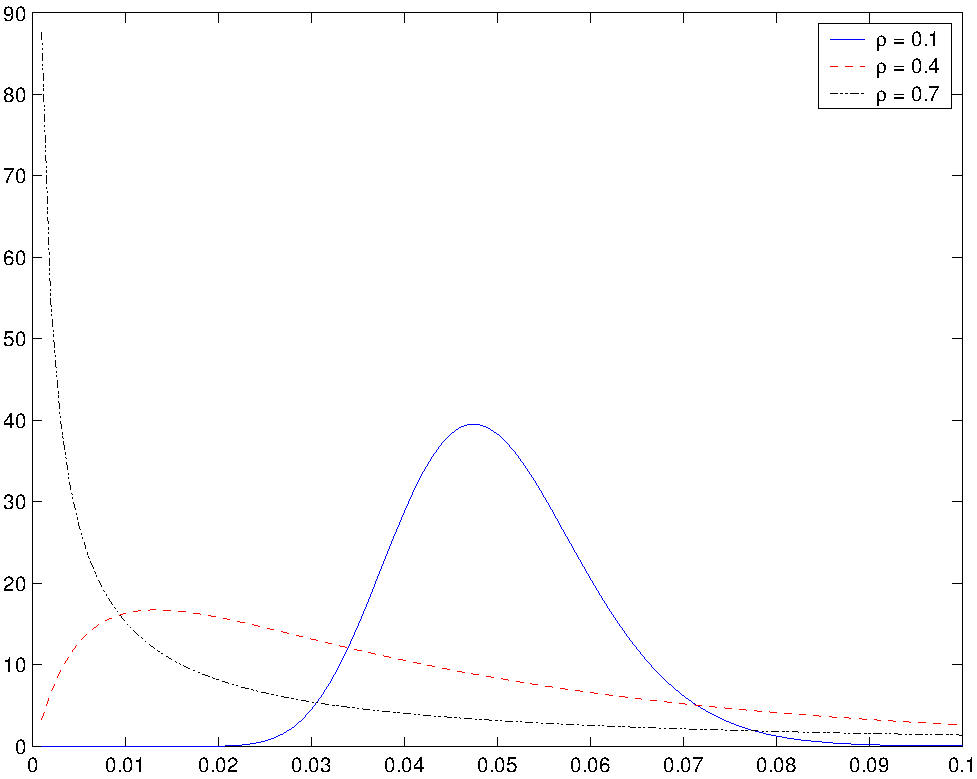
\includegraphics[width=0.8\textwidth]{./Figures/dens.pdf}
\caption{The density function $f$ as given in \eqref{density} for
  three different $\rho$'s and $\bar{p} = 0.05$. (Plotted on $[0,
  0.1]$ for convenience.)}
\label{fig:dens2}
\end{center}
\end{figure}


Let's see one more result on Table~\ref{tab:data}. According to~\cite{Fraz06}\ldots

% Table generated by Excel2LaTeX from sheet 'Sheet1'
\begin{table}
\caption{These are the data.} \label{tab:data}
\begin{center}
\begin{tabular}{l|rrrrrl}
\hline \hline
DJ CDX Tranches: &      0-3\% &      3-7\% &     7-10\% &    10-15\% &    15-30\% &       RMSE \\

Market mid spread &    40.00\% &      312.5 &      122.5 &       42.5 &       12.5 &            \\

Bid/Ask Spread &     2.00\% &         15.0 &          7 &          7 &          3 &            \\

Stochastic vol intensities &    41.80\% &      308.9 &      116.2 &       44.9 &          2 &       1.68 \\

Jump-diffusion intensities &    46.90\% &      340.2 &      119.7 &       61.9 &       14.3 &       2.17 \\

Pure-diffusion intensities &    49.30\% &      442.9 &       94.9 &       16.8 &        0.4 &       5.34 \\

Gaussian copula &    46.80\% &      474.4 &      131.8 &       36.9 &        2.9 &        5.3 \\

RFL Gaussian copula &    48.60\% &      334.9 &      125.5 &       66.5 &        9.2 &       2.59 \\

Double-t copula &    45.10\% &        367 &      114.9 &       54.9 &         20 &       2.44 \\
\hline \hline
\multicolumn{ 6}{l}{Source: Some source that I quote in the form Author (YYYY).} &

\end{tabular}
\end{center}
\end{table} 
